The convolutional neural networks described above will progressively reduce the size of the image (through pooling) and then classify the image as a whole. For segmentation, we need each pixel in the image to be classified, thus the output needs to be the same size as the input. 


\begin{figure}[h!]
\centering
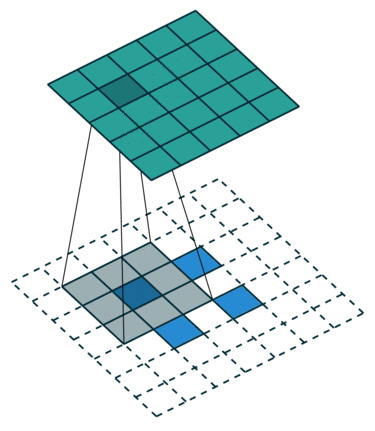
\includegraphics[scale=0.45]{pictures/deConv}
\caption{Image showing a deconvolution operation, where the input is in blue, the ouput is in cyan and the weight matrix is the shaded region. The original input is a 2x2 region, which is padded with zeros in order to produce an output which is larger \cite{convPics}.}
\label{fig:deConv}
\end{figure}

Long et al. have produced a convolutional neural network architecture that is capable of producing accurate segmentation \cite{fcn}. The network is a fully convolutional network (FCN), that is, all layers are either convolutional or pooling layers, with activation functions. The first part of the network works similarly to what is described above. However, the network also has what is usually referred to as \textit{deconvolution layers}, which produces an output that is larger than its input. Deconvolution is in reality just the same operation as convolution, but with a fractional stride. This is  achieved by enlarging the input by adding in zero valued pixels, and performing a regular convolution operation (see figure \ref{fig:deConv}). One can then re-produce an output of the same size as the original image by the end of the network, thus giving class labels for each individual pixel. Long et al. also find that they achieved better results by combining the results of multiple different layers. By doing this, they can combine the coarser information of the later layers with the more fine details of the earlier layers to achieve good results.

There is another way around this, as done in the DeepIGeoS network \cite{deepIGeoS}. This time, the FCN does not gradually reduce the size of the original input through pooling, but instead extracts progressively larger features through \textit{dilated convolution}. In this case, the weight matrix, rather than the input, is enlarged by padding it out with zeros, such that the receptive field is progressively enlarged. Similarly to Long et al., DeepIGeoS then combines the predictions from the different layers via channel concatenation in order to consider both the large scale features and the finer details. They find that this is an improvement over only considering the final layer. 

In the case of Long et al., information is progressively destroyed as the image becomes coarser and the deconvolution layers attempt to re-construct it. In the case of DeepIGeoS however, the information is never destroyed, instead, progressively larger features are extracted via dilated convolution.